\documentclass[german,a4paper]{beamer}
\usepackage[ngerman]{babel}
\usetheme{Warsaw}  %% Themenwahl
\usepackage{beamerprosper} 
\usepackage{amsmath}
\usepackage{colortbl}
\usepackage{graphicx}

\title{IPA 1. Meilstein Präsentation}
\author{Marius Oppolzer \and Matthieu Grillere}
\date{\today}
 
\begin{document}
\maketitle{}
\begin{frame}
\frametitle{Inhaltverzeichnis}
\tableofcontents[pausesections]
\end{frame}
 
\section{Einf\"{u}rung in Li-Fi}
\subsection{Einf\"{u}rung}
\begin{frame} 
\frametitle{Einf\"{u}rung}
\begin{itemize}
  \item 
  Software für interaktive Vorträge
  \item
  Großveranstaltungen ungefähr 1000 Teilnehmer
  \item
  online Kommunikation
  \item
  Umfragen, Fragen, Temporegulierung
\end{itemize}
\end{frame}

\subsection{Grundidee}
\begin{frame} 
\frametitle{Technisches}
\begin{itemize}
  \item 
  3 Komponenten
  \begin{itemize}
    \item
    Serverseitiges Backend
    \item
    Frontend Webbrowser
    \item
    Fronten Adroid-API
  \end{itemize}
  \item 
  REST API
  \item
  Socket IO
  \item
  Eigenschaften
  \begin{itemize}
    \item
    HTML5 und CCS3
    \item
    AndroidApp für Android Version ab 4.0
  \end{itemize}
\end{itemize}
\end{frame}

\begin{frame} 
\frametitle{Konzept}
\begin{itemize}
  \item{}
  3 Rollen: Teilnehmer (default), Dozent, Administrator
  \item
  Teilnehmer kann an bestehenden Veranstaltungen teilnehmen
  \item{}
  Dozent kann Veranstaltung leiten oder teilnehmen
  \item{}
  1 Administrator im System 
\end{itemize}
\end{frame}

\section{Funktionsbeschreibung}
\subsection{Allgemein}
\begin{frame} 
\frametitle{Allgemeine Funktionen}
\begin{itemize}
  \item{}
  Registrieren / Anmelden \\
  \quad \emph{Rechte : -}
  \item{} 
  Abmelden  \\
  \quad \emph{Rechte : -}
\end{itemize}
\end{frame}

\subsection{Teilnehmer}
\begin{frame} 
\frametitle{Teilnehmer Funktionen}
\begin{itemize}
  \item{}
  Veranstaltung beitreten \\
  \quad \emph{Rechte : join\_lecture}
  \item{} 
  Veranstaltung verlassen  \\
  \quad \emph{Rechte : leave\_lecture}
  \item{} 
  Umfrage abstimmen  \\
  \quad \emph{Rechte : vote\_survey}
  \item{} 
  Regulierung des Vortragstempos  \\
  \quad \emph{Rechte : regulate\_speed}
  \item{} 
  Frage stellen  \\
  \quad \emph{Rechte : create\_question}
  \item{} 
  Frage best\"{a}tigen  \\
  \quad \emph{Rechte : vote\_question}
  \item{} 
  Frage einsehen  \\
  \quad \emph{Rechte : view\_question}
\end{itemize}
\end{frame}

\subsection{Dozent}
\begin{frame} 
\frametitle{Dozent Funktionen}
\begin{tabular}{p{5,5cm} p{6cm}}
    \begin{itemize}
    \item{}
    Veranstaltung erstellen \\
    \quad \emph{Rechte : manage\_lecture}
    \item{}
    Veranstaltung beenden (nicht verlassen!) \\
    \quad \emph{Rechte : manage\_lecture}
    \item{}
    Umfrage erstellen \\
    \quad \emph{Rechte : create\_survey}
    \item{}
    Umfrage speichern \\
    \quad \emph{Rechte : create\_survey}
    \item{}
    Umfrage freigeben \\
    \quad \emph{Rechte : create\_survey}
    \end{itemize}
  &
    \begin{itemize}
    \item{}
    Umfrage beenden \\
    \quad \emph{Rechte : close\_survey}
    \item{}
    Umfrage auswerten \\
    \quad \emph{Rechte : view\_survey} 
    \item{}
    Vortragstempo einsehen \\
    \quad \emph{Rechte : view\_speed}
    \item{}
    Frage einsehen \\
    \quad \emph{Rechte : view\_question}
    \item{}
    Frage l\"{o}schen \\
    \quad \emph{Rechte : delete\_question}
    \end{itemize}
\end{tabular}

\end{frame}

\subsection{Admin}
\begin{frame} 
\frametitle{Admin Funktionen}
\begin{itemize}
  \item{}
  Account erstellen \\
  \quad \emph{Rechte : create\_account}
  \item{} 
  Account l\"{o}schen  \\
  \quad \emph{Rechte : delete\_account}
  \item{} 
  Rolle zuweisen  \\
  \quad \emph{Rechte : assign\_role}
  \item{} 
  Rolle anlegen  \\
  \quad \emph{Rechte : create\_role}
  \item{} 
  Rolle modifizieren  \\
  \quad \emph{Rechte : edit\_role}
  \item{} 
  Rolle l\"{o}schen  \\
  \quad \emph{Rechte : delete\_role}
\end{itemize}
\end{frame}

\section{Rollen und Rechte}
\begin{frame} 
\frametitle{\"{U}bersicht von Rollen und Rechten}
\resizebox{11,5cm}{!} {
  \begin{tabular}{c<{\onslide<2->} c<{\onslide<3->}c<{\onslide}c}
  \textbf{Teilnehmer} & \textbf{Dozent} & \textbf{Administrator} \\
  create\_question  & \emph{Teilnehmerrechte (ohne leave\_lecture)} & \emph{Teilnehmer und Dozentrechte} \\
  view\_question & create\_survey & config \\
  vote\_question & close\_survey & create\_account\\
  join\_lecture & view\_speed & delete\_account \\
  leave\_lecture & view\_survey & assign\_role \\
  regulate\_speed & manage\_lecture & create\_role \\
  vote\_survey & & edit\_role \\
  & & delete\_role \\
  \end{tabular}
}
\end{frame}

\section{Verhalten}
\subsection{Aktivit\"{a}tsdiagramm}
\begin{frame}
\frametitle{Veranstaltung verwalten}
\includegraphics[width=1.0\textwidth]{ad_VA_verwalten.jpg}
\end{frame}

\begin{frame}
\frametitle{Dozent Diagramm}
\includegraphics[width=1.0\textwidth]{AD_Admin.jpg}
\end{frame}

\subsection{Datenbank}
\begin{frame}
\frametitle{E-R Diagramm}
\includegraphics[width=1.0\textwidth]{er-diagram.png}
\end{frame}

\section{Mockup}
\subsection{Android App}
\subsection{Desktop Version}
\end{document}
